\documentclass[10pt,a4paper]{article}
\usepackage[utf8]{inputenc}
\usepackage[german]{babel}
\usepackage[T1]{fontenc}
\usepackage{amsmath}
\usepackage{amsfonts}
\usepackage{amssymb}
\usepackage{float}
\usepackage{graphicx}
\renewcommand\thesubsection{\alph{subsection}}
\begin{document}

\begin{center}
\begin{LARGE}
Differentialgleichungen
\end{LARGE}

Modellierung Dynamischer Systeme: Praktikum 1

Johannes Reidl, Sigurd Sippel

\end{center}

\section{Lösung  "`steifer Differentialgleichungen"' mit Euler/Runge-Kutta (RK 2. Ordng.)}

\subsection{Geben Sie das Analogrechner-/Simulink-Schaltbild an.}
\begin{figure}[H]
\centering
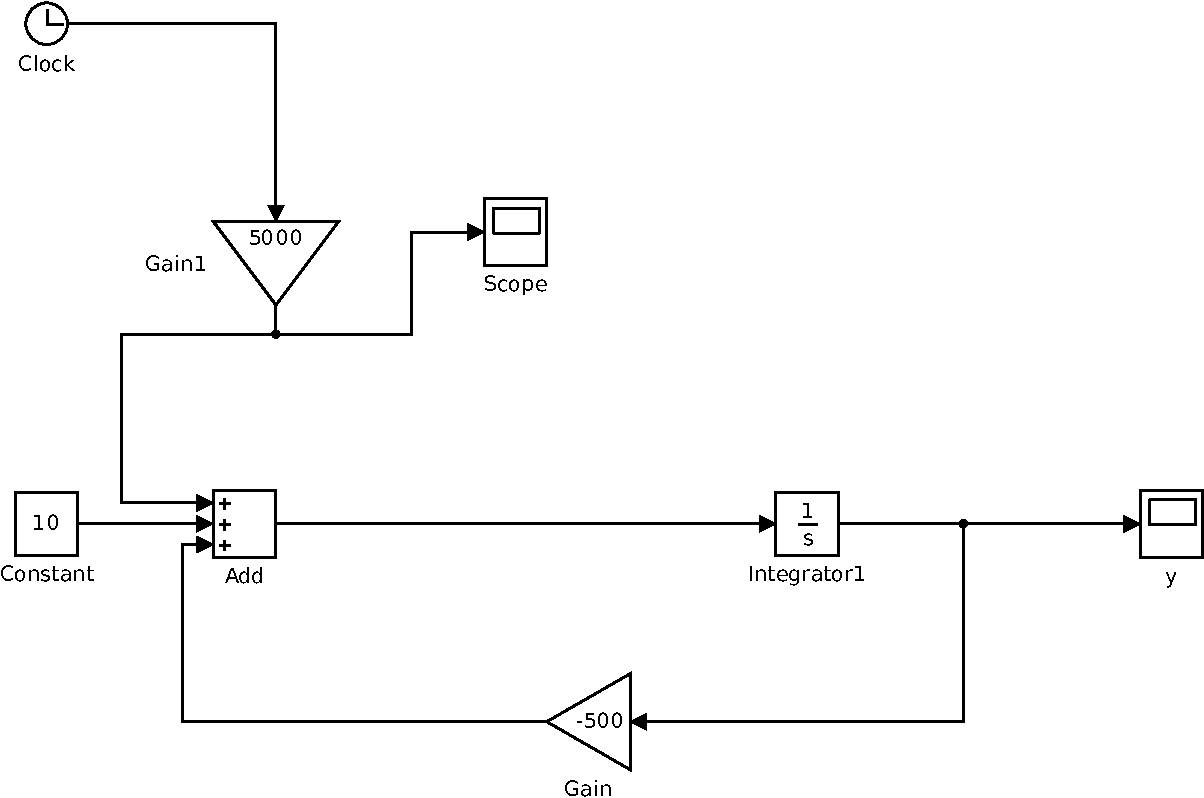
\includegraphics[width=0.9\linewidth]{../screenshots/1}
\end{figure}
\subsection{Geben Sie die Iterationsgleichungen für das Euler-Verfahren an.}
\begin{subequations}
\begin{align}
y_{n+1} = y_n + h * y'(x_n,y_n)\\
x_{n+1} = x_n + h
\end{align}
\end{subequations}

\subsection{Geben Sie die Iterationsgleichungen für das RK2-Verfahren an.}
\begin{subequations}
\begin{align}
k1 = h * y'(x_n,y_n)\\
k2 = h * y'(x_n + \frac{h}{2},y_n + \frac{k1}{2})\\
y_{n+1} = y_n + k2\\
x_{n+1} = x_n + h
\end{align}
\end{subequations}

\subsection{Geben Sie die Iterationsgleichungen für das implizite Euler-Verfahren an.}
\begin{subequations}
\begin{align}
y_{n+1} = y_n + h * (10 - 500 * y_{n+1} + 5000 * x_{n+1})\\
y_{n+1} = y_n + 10 * h - 500 * y_{n+1} * h + 5000 * x_{n+1} * h)\\
y_{n+1} + 500 * y_{n+1} * h = y_n + 10 * h + 5000 * x_{n+1} * h)\\
y_{n+1} * (1+ 500 * h) = y_n + 10 * h + 5000 * x_{n+1} * h)\\
y_{n+1} = \frac{(y_n + 10 * h + 5000 * h * x_n+1)}{ (1+500*h)}
\end{align}
\end{subequations}

\subsection{Schreiben Sie ein Programm "`Stiff.ch"', welches die DGL mit allen Verfahren
löst und zusammen mit der analytischen Lösung in einem Plot anzeigt.}

Die Implementierung ist in Stiff.ch zu finden.

Bei einer Schrittweite von $h = 0.0001$ sind alle Verfahren ziemlich gut, dennoch ist der Euler am weitesten von der analytischen Funktion entfernt.
\begin{figure}[H]
\centering
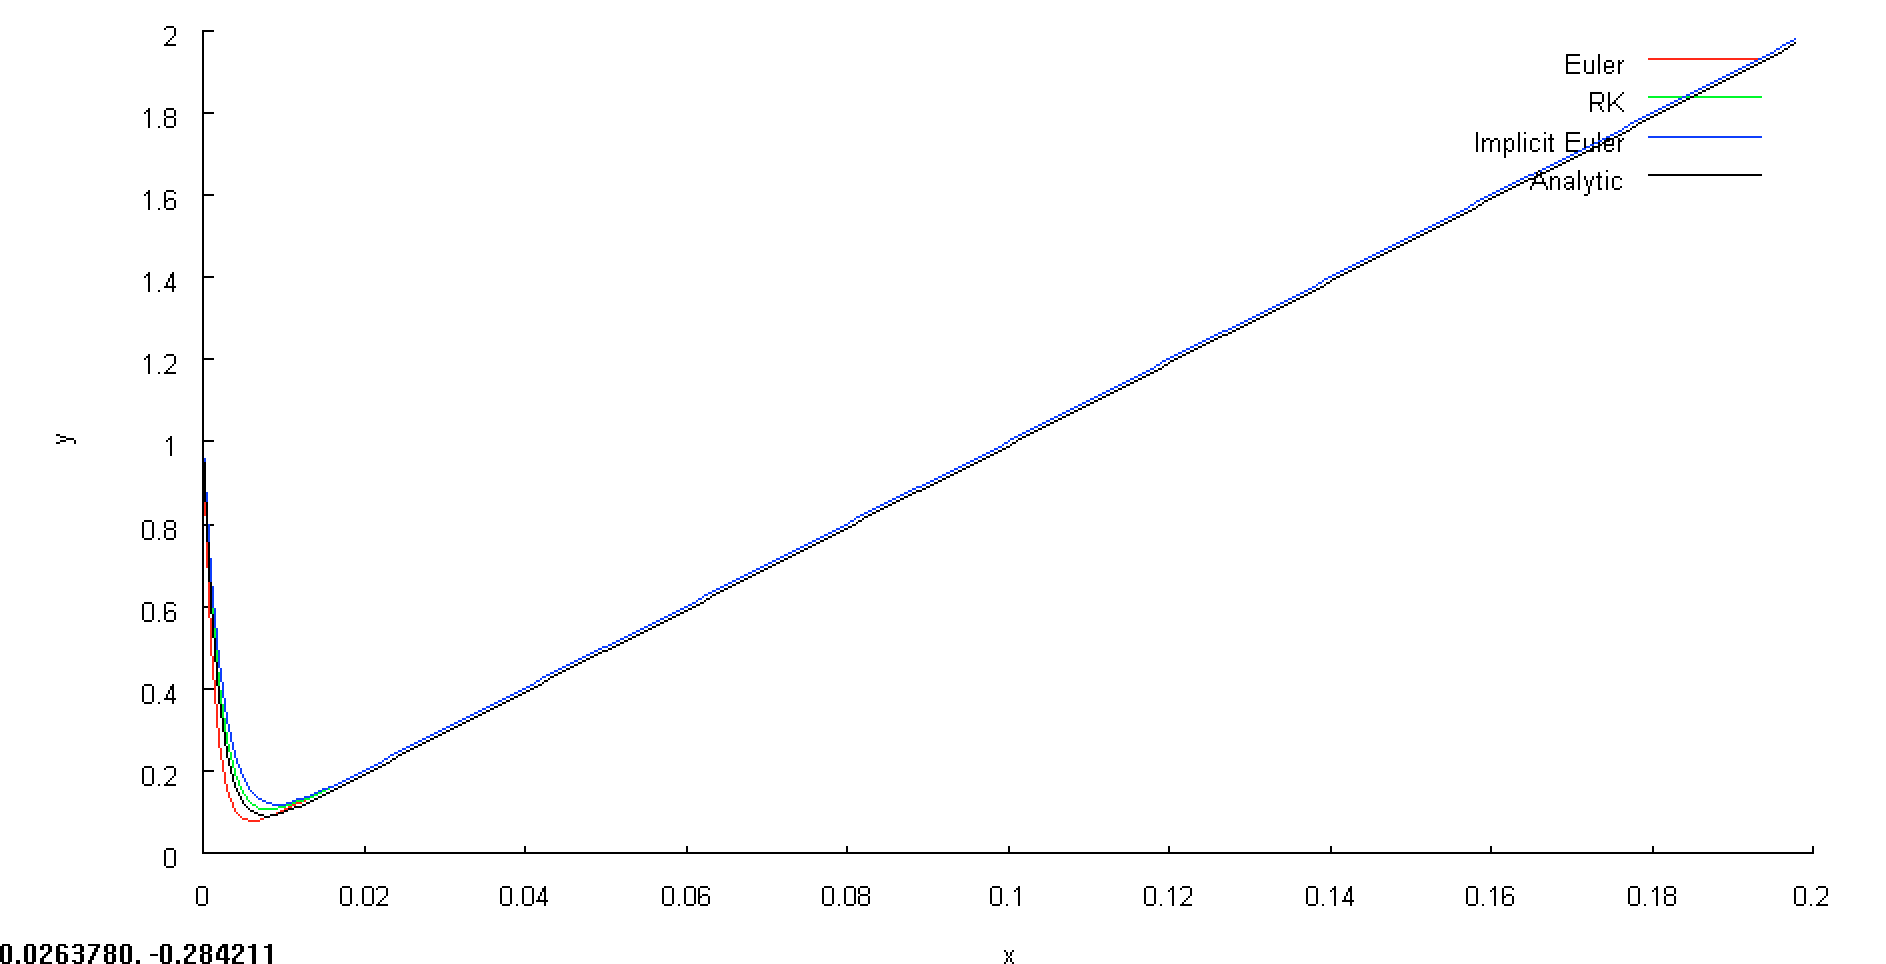
\includegraphics[width=0.9\linewidth]{../screenshots/stiff0001.png}
\end{figure}
Bei einer Schrittweite von $h = 0.0001$ schwingt der Euler sehr stark, jedoch normalisiert sich die Darstellung mit steigendem X-Wert. Implizit Euler und RK sind gut.
\begin{figure}[H]
\centering
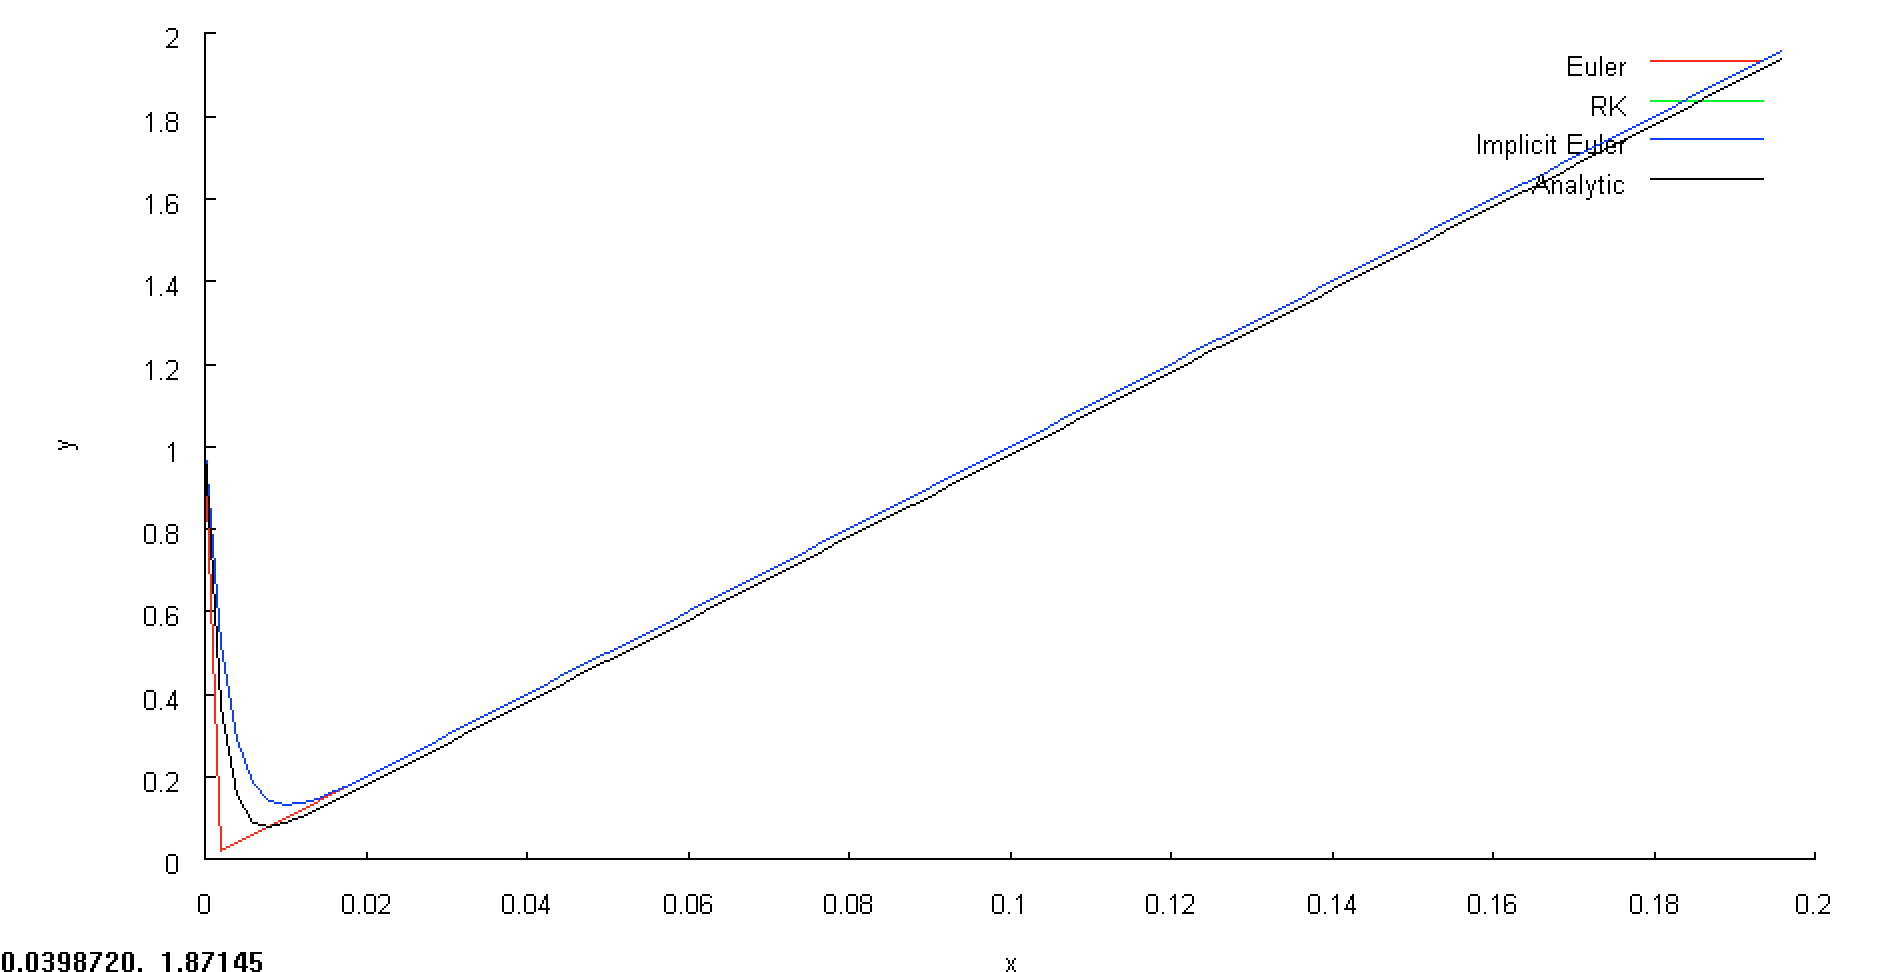
\includegraphics[width=0.9\linewidth]{../screenshots/stiff0002.png}
\end{figure}
Bei einer Schrittweite von $h = 0.0002$ zeigt Euler keine Kurve mehr, RK und Implizit Euler zeigen eine gute Darstellung.
\begin{figure}[H]
\centering
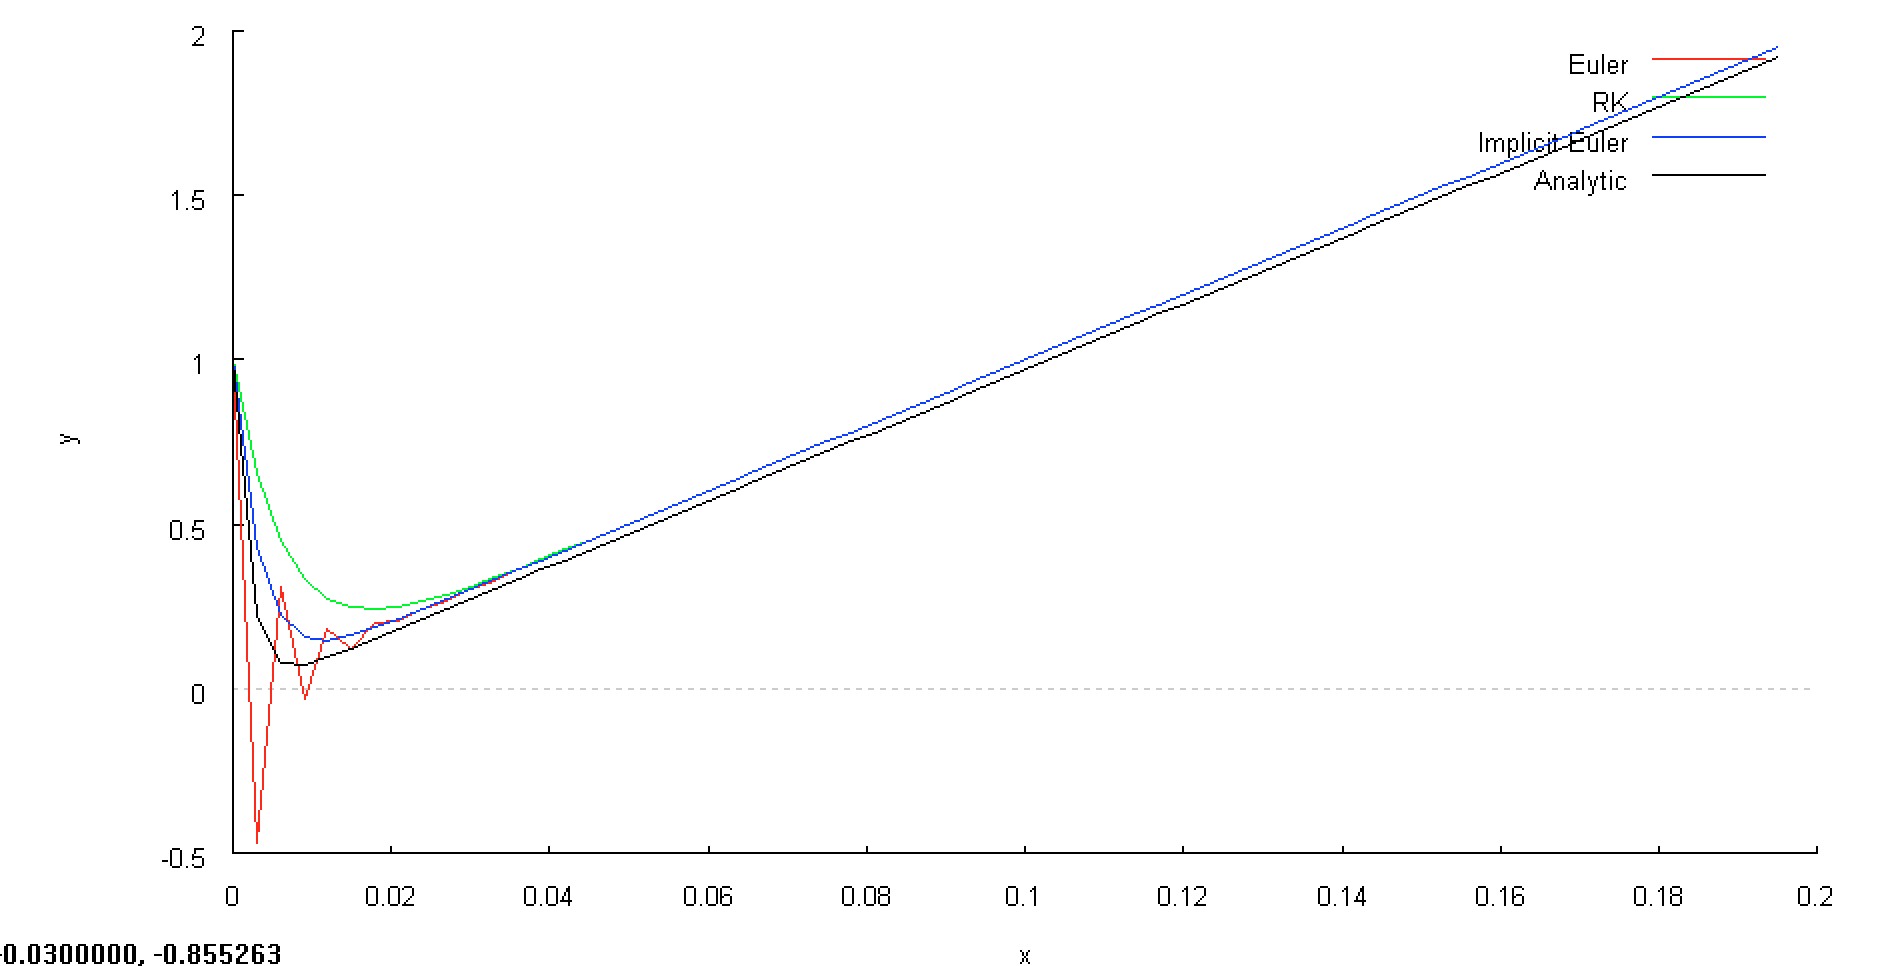
\includegraphics[width=0.9\linewidth]{../screenshots/stiff0003.png}
\end{figure}
Bei einer Schrittweite von $h = 0.0003$ schwingt der Euler sehr stark. RK und Implizit Euler zeigen eine gute Darstellung.
\begin{figure}[H]
\centering
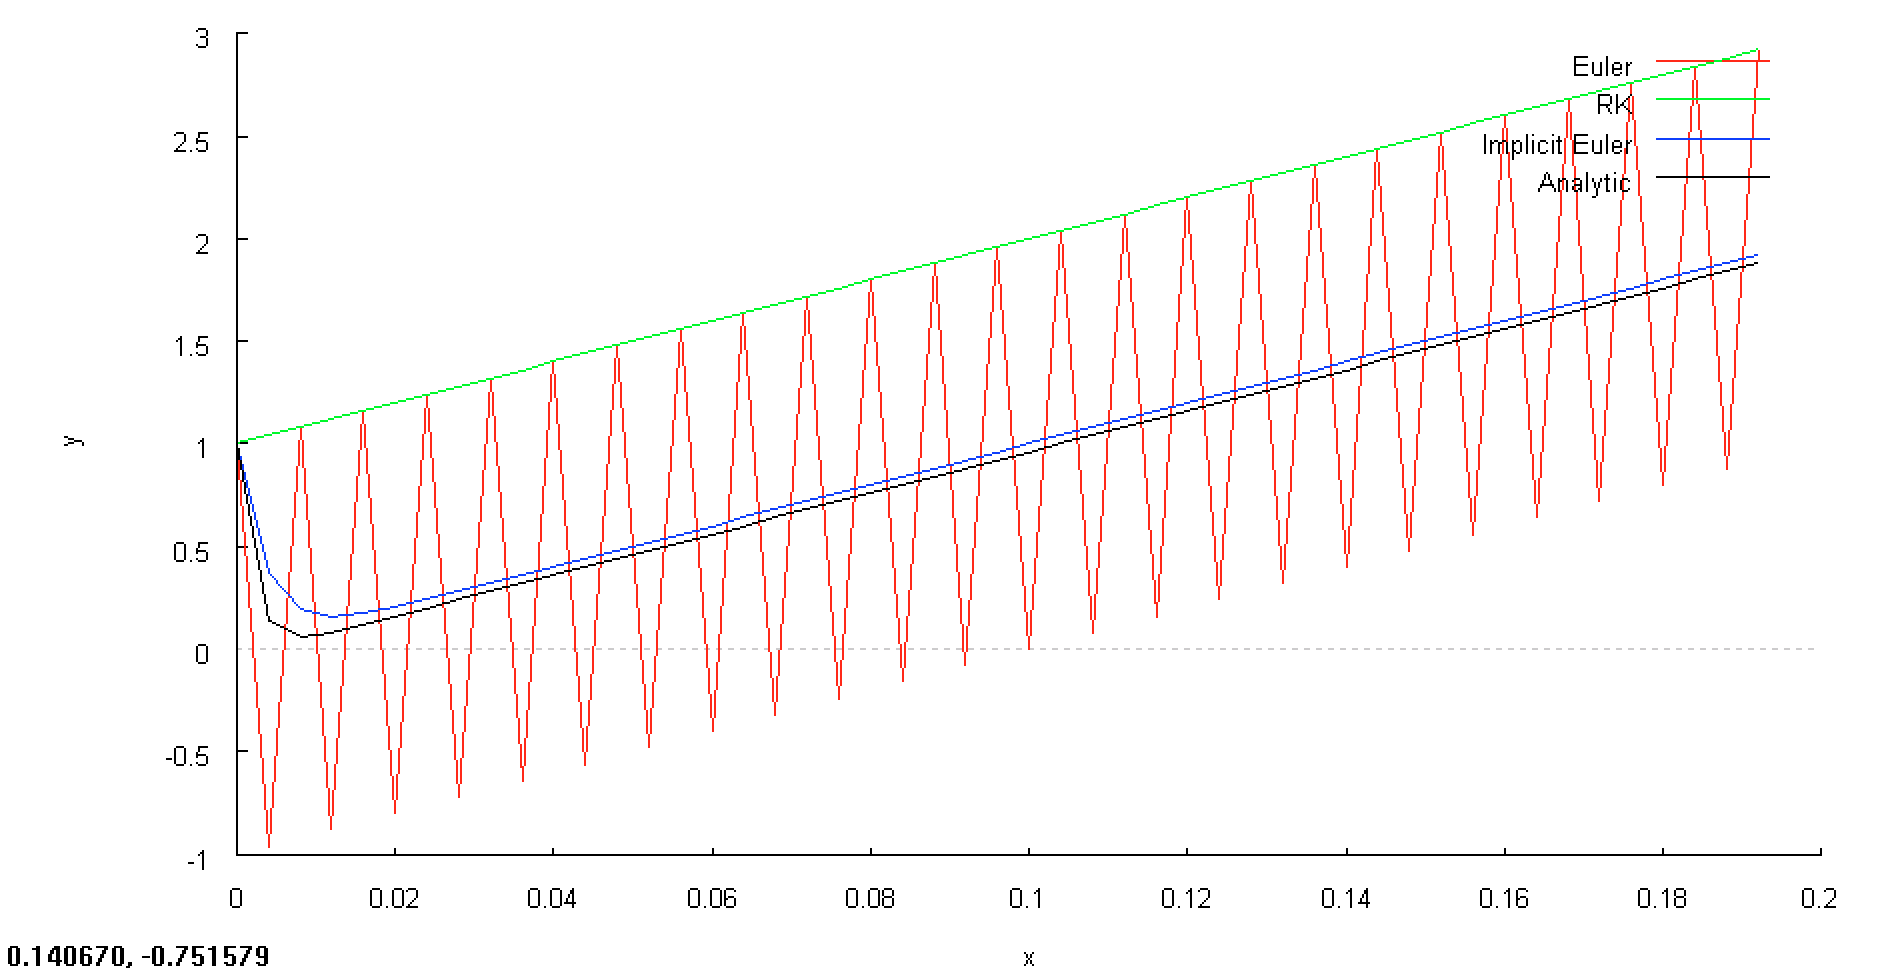
\includegraphics[width=0.9\linewidth]{../screenshots/stiff0004.png}
\end{figure}
Bei einer Schrittweite von $h = 0.0004$ schwingt der Euler kontinuerlich, RK zeigt nur noch eine Gerade. Implizit Euler zeigt eine gute Darstellung.
\begin{figure}[H]
\centering
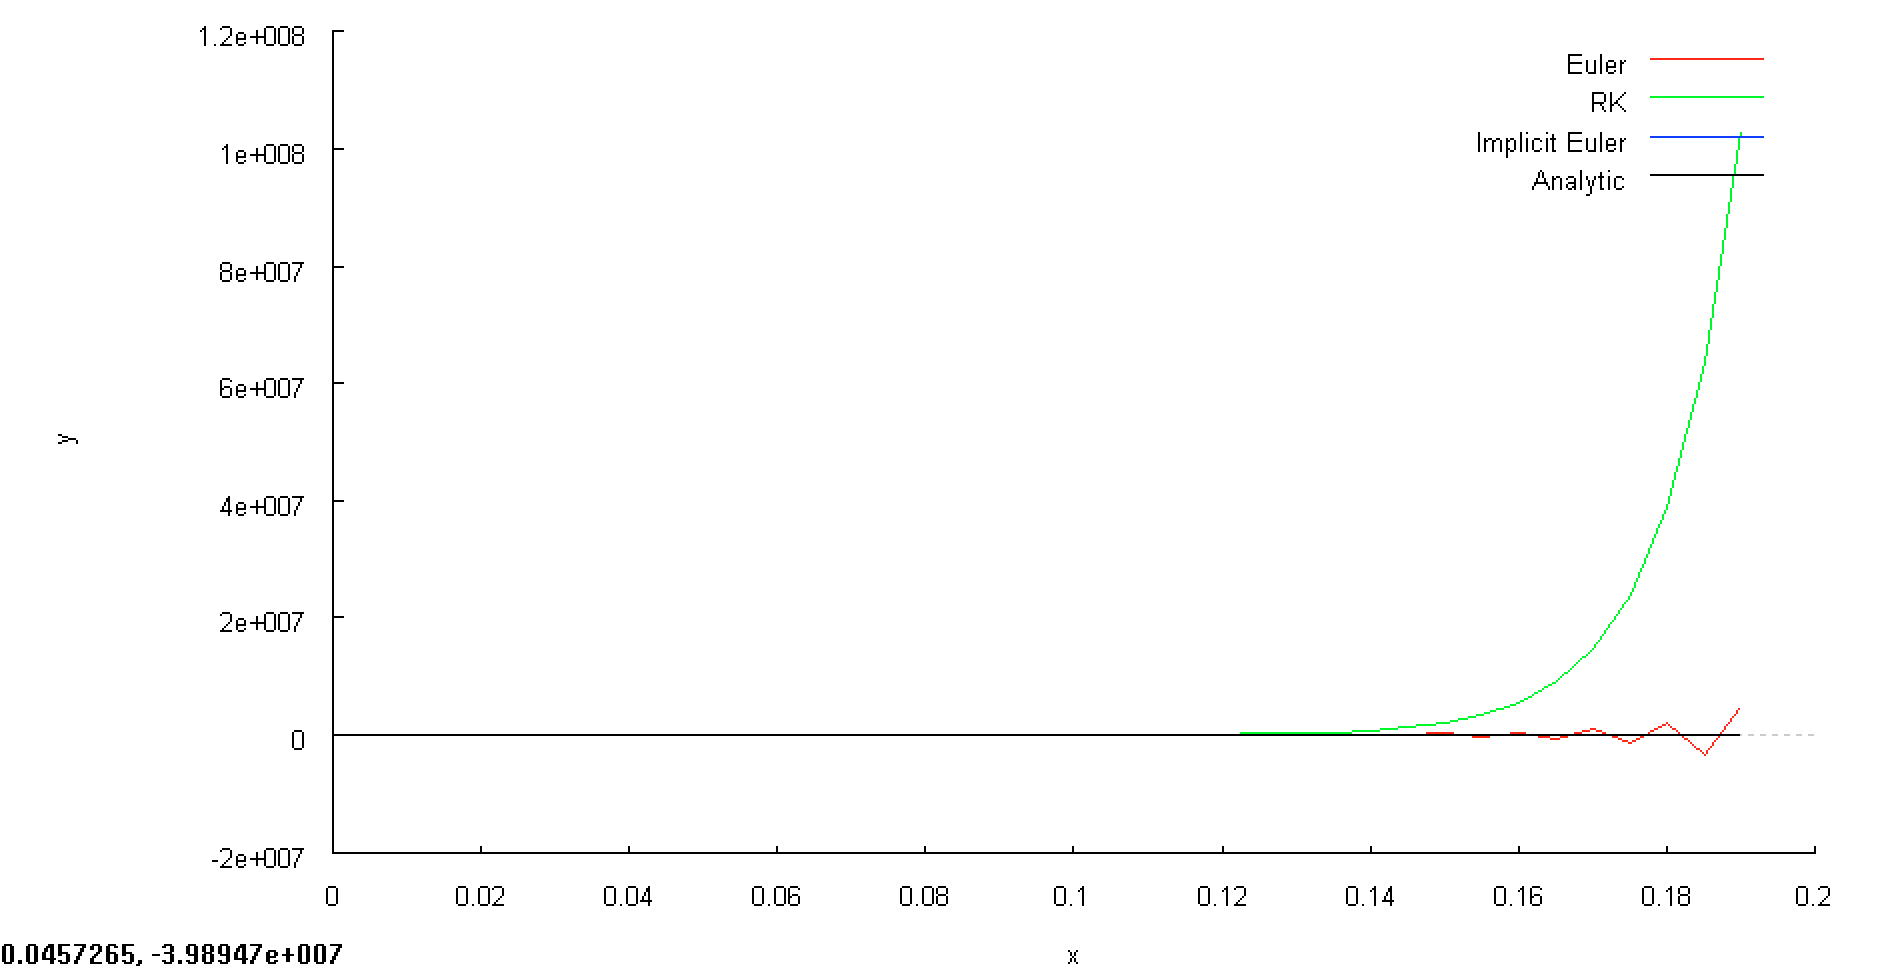
\includegraphics[width=0.9\linewidth]{../screenshots/stiff0005.png}
\end{figure}
Bei $h = 0.0005$ werden die Y-Werte des RK sehr hoch.

\section{Lösung einer (nichtlinearen) DGL 2. Ordnung (Van-der-Pol-DGL) mit RK 2}
\subsection{Geben Sie das Analogrechner-/Simulink-Schaltbild an.}
\begin{figure}[H]
\centering
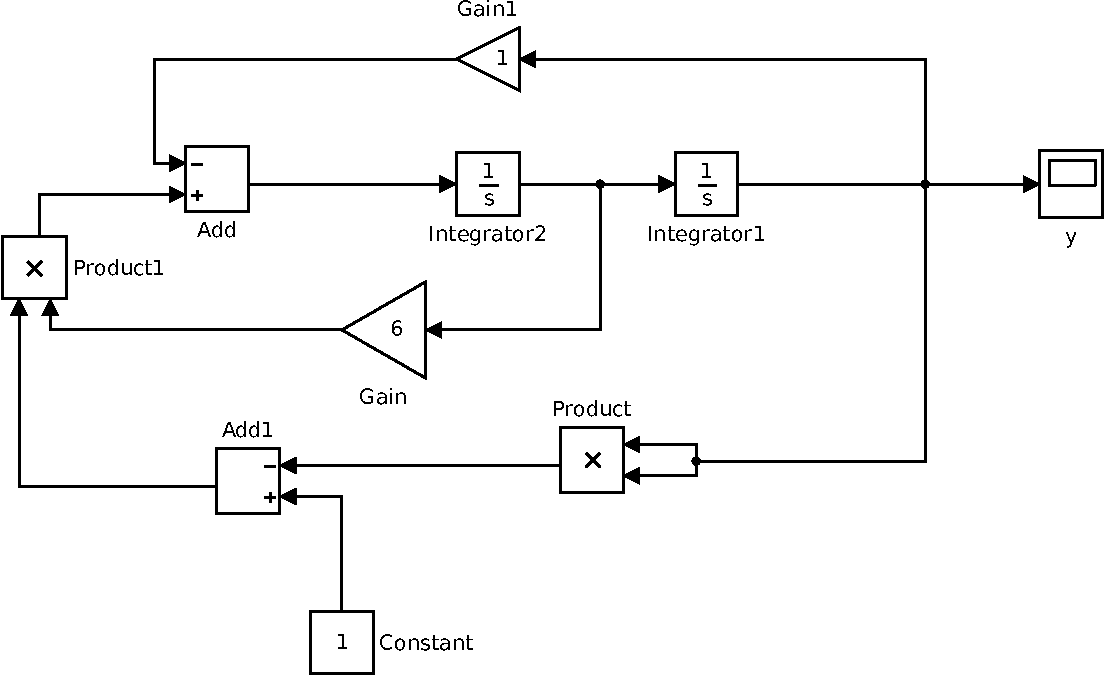
\includegraphics[width=0.9\linewidth]{../screenshots/2}
\end{figure}

\subsection{Geben Sie die DGL 2. Ordnung als 2 DGLn 1. Ordnung an.}

Zerlegung der DGL $y'$ in $y1'$ und $y2'$:
\begin{align}
y'' = 6 * (1-y^2) * y' - y
\\y1' = 6 * (1-y2^2) * y1 - y2
\\y2' = y1
\end{align}

\subsection{Geben Sie die Iterationsgleichungen für das Euler-Verfahren an.}

\begin{align}
y1_{n+1} = y1_n + h * y1'(y1_n,y2_n)
\\y2_{n+1} = y2_n + h * y2'(y2_n)
\\x_{n+1} = x_n + h
\end{align}

\subsection{Geben Sie die Iterationsgleichungen für das RK2-Verfahren an.}

\begin{align}
k1 = h * y1'(y1_n, y2_n);
\\l1 = h * y2'(y1_n);
\\k2 = h * y1'(y1_n + l1/2, y2_n + l1/2);
\\l2 = h * y2'(y1_n + k1/2);
\\y1_{n+1} = y1_n + k2
\\y2_{n+1} = y2_n + l2
\\x_{n+1} = x_n + h
\end{align}

\subsection{Schreiben Sie ein Programm "VanDerPol.ch", welches die DGL mit beiden
Verfahren löst und in einem Plot anzeigt.}

Die Implementierung ist in VanDerPol.ch zu finden.

Der Plot zeigt bei einer Schrittweite von $h = 0.001$ bei Euler und RK eine sehr genaue Darstellung.

\begin{figure}[h]
\centering
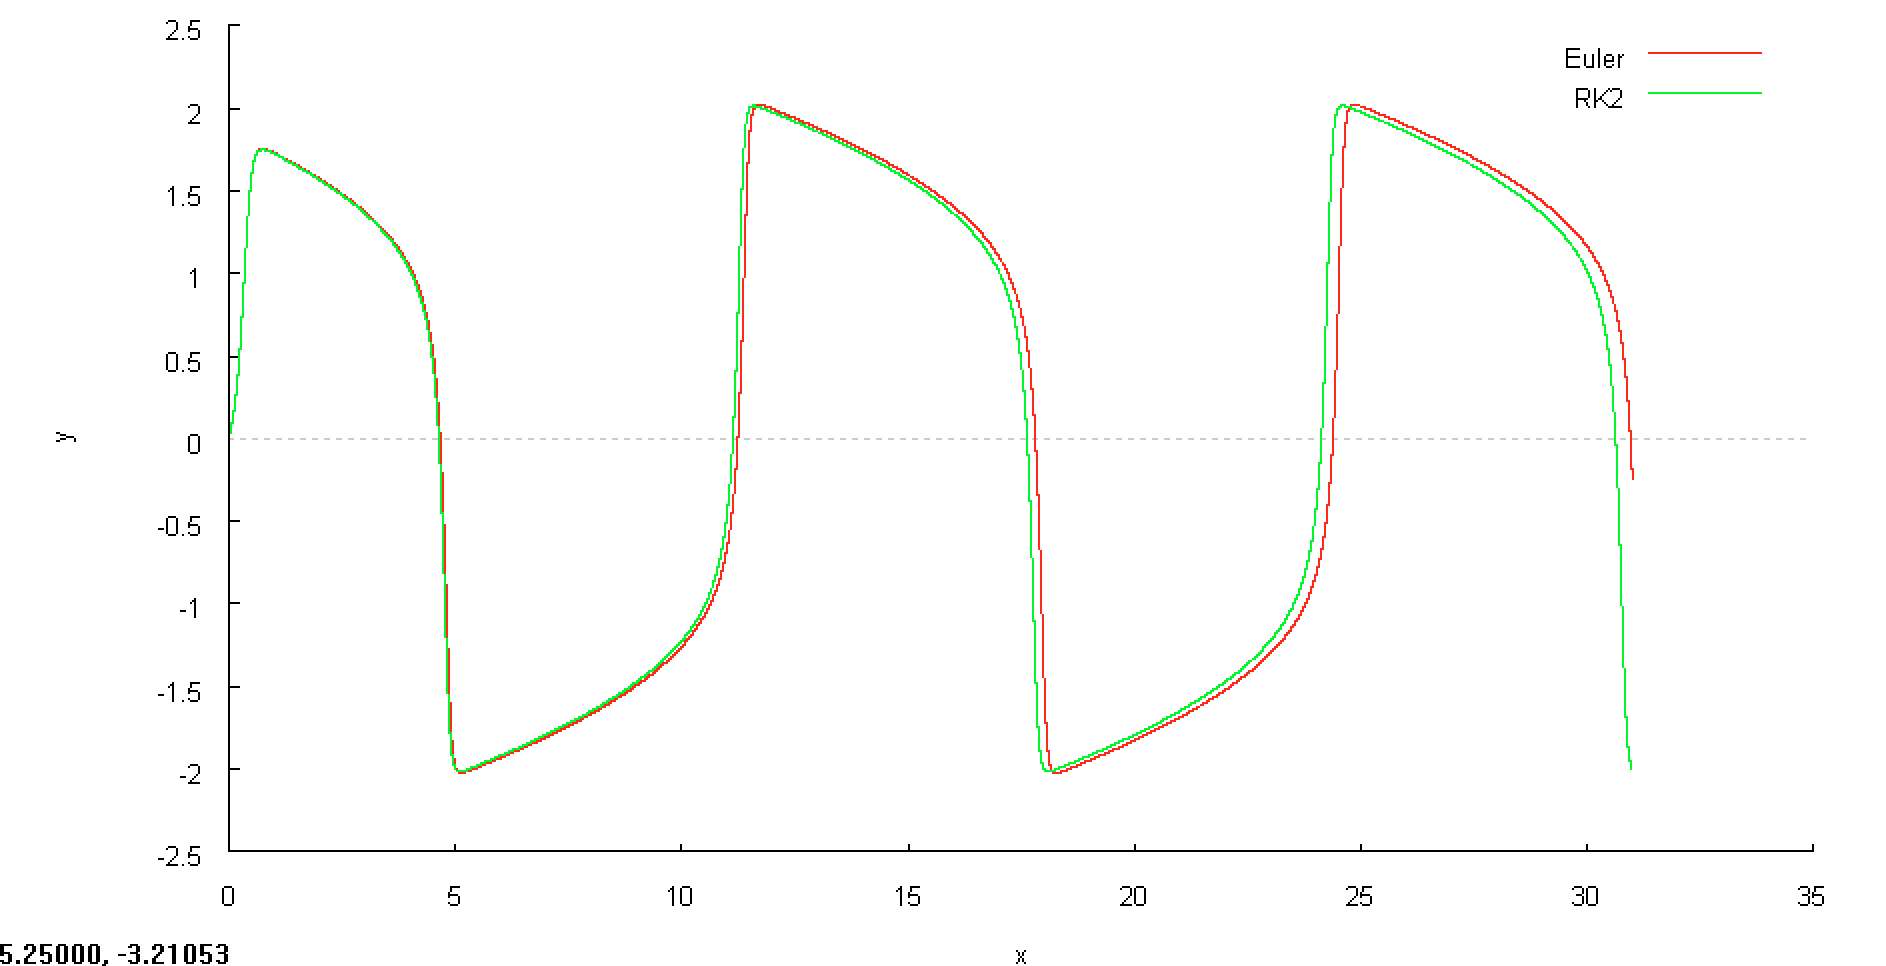
\includegraphics[width=0.9\linewidth]{../screenshots/van001.png}
\end{figure}
Bei einer Schrittweite von $h = 0.2$ sind Euler und RK sehr ungenau, wobei RK noch etwas näher an der korrekten Darstellung ist.
\begin{figure}[h]
\centering
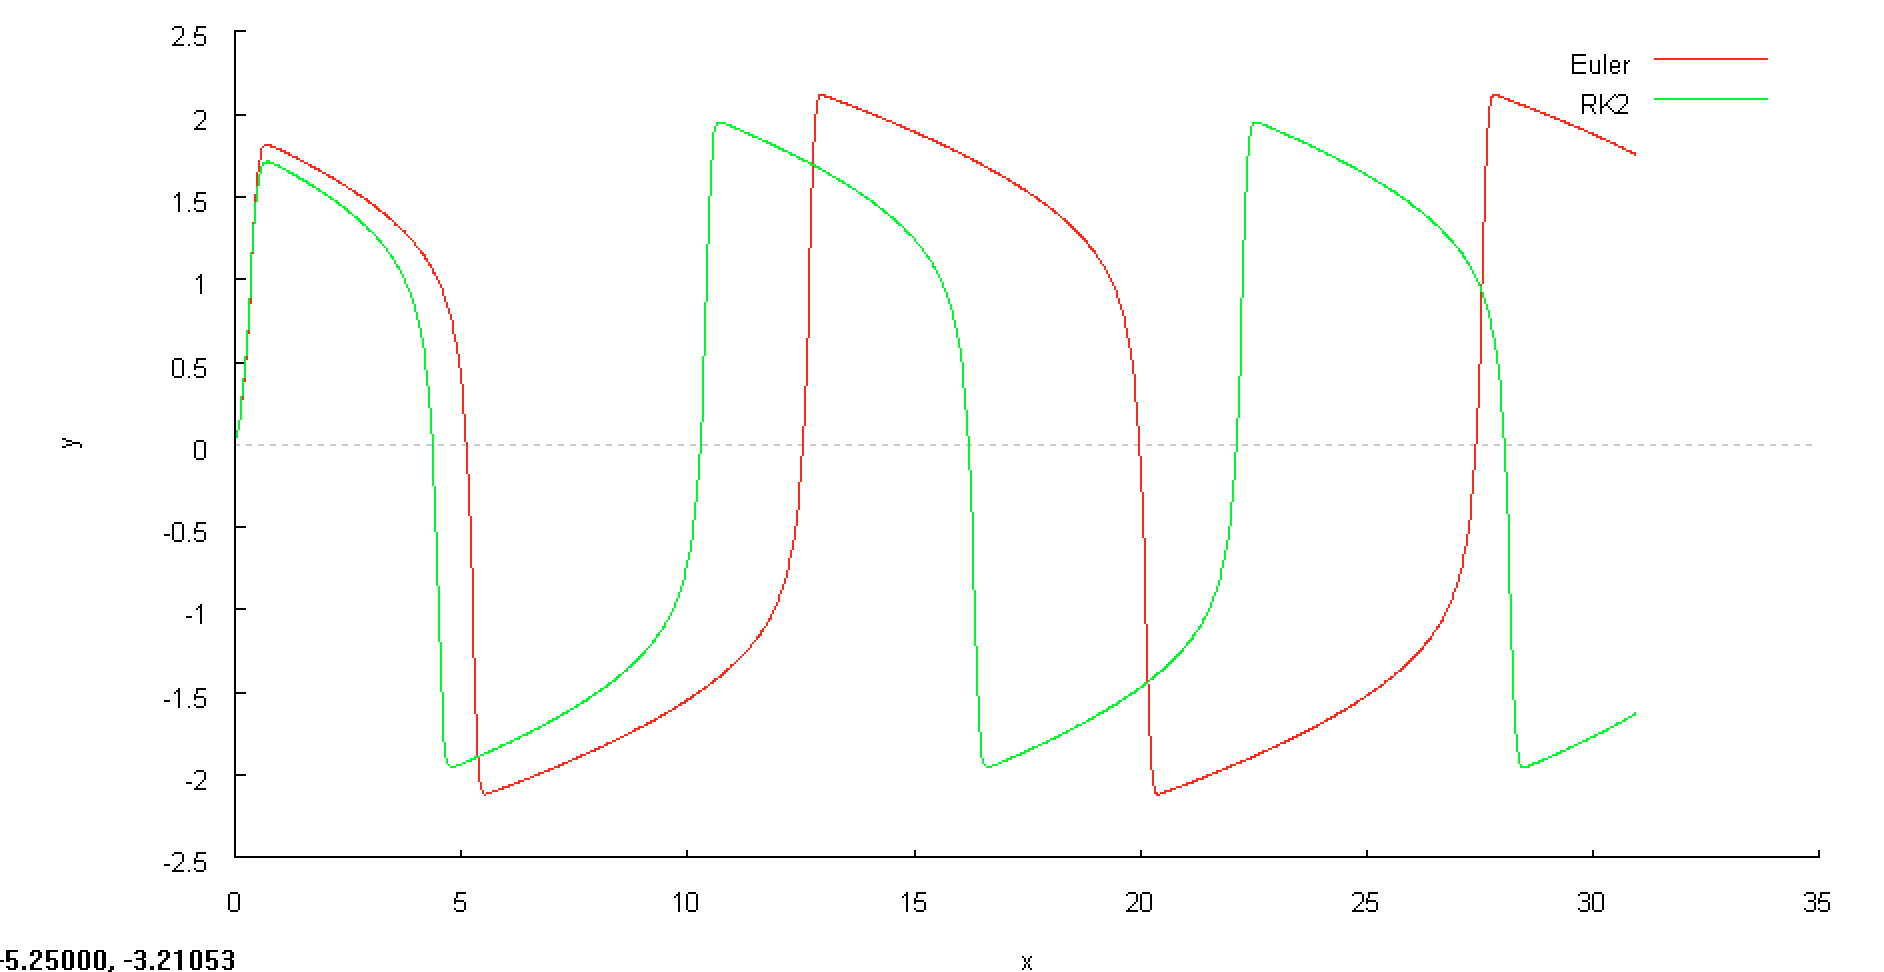
\includegraphics[width=0.9\linewidth]{../screenshots/van02.png}
\end{figure}

\section{Lösung eines Differentialgleichungssystems (Lorenz-Attraktor) mit RK 2}
\subsection{Geben Sie die Iterationsgleichungen für das RK2-Verfahren an.}
\begin{subequations}
\begin{align}
k_{1x} = -10 * h * (x_n - y_n)\\
k_{1y} = h * [(40-z_n) * x_n - y_n]\\
k_{1z} = h * [(x_n * y_n) - (2,67 * z_n)]\\
k_{2x} = -10 * h * [(x_n +\frac{k_{1x}}{2}) - (y_n + \frac{k_{1y}}{2})]\\
k_{2y} = h * [(40 - z + \frac{k_{1z}}{2}) * (x + \frac{k_{1x}}{2}) - (y_n + \frac{k_{1y}}{2})]\\
k_{2z} = h * [(x + \frac{k_{1x}}{2}) * (y + \frac{k_{1_y}}{2}) - 2,67 * (z + \frac{k_{1z}}{2})]
\end{align}
\end{subequations}

\subsection{Schreiben Sie ein Programm "Lorenz.ch", welches das DGL-System löst.
Geben Sie im 1. Plot die Funktion x(t) aus:
Geben Sie im 2. Plot z(x) aus.}

\begin{figure}[H]
\centering
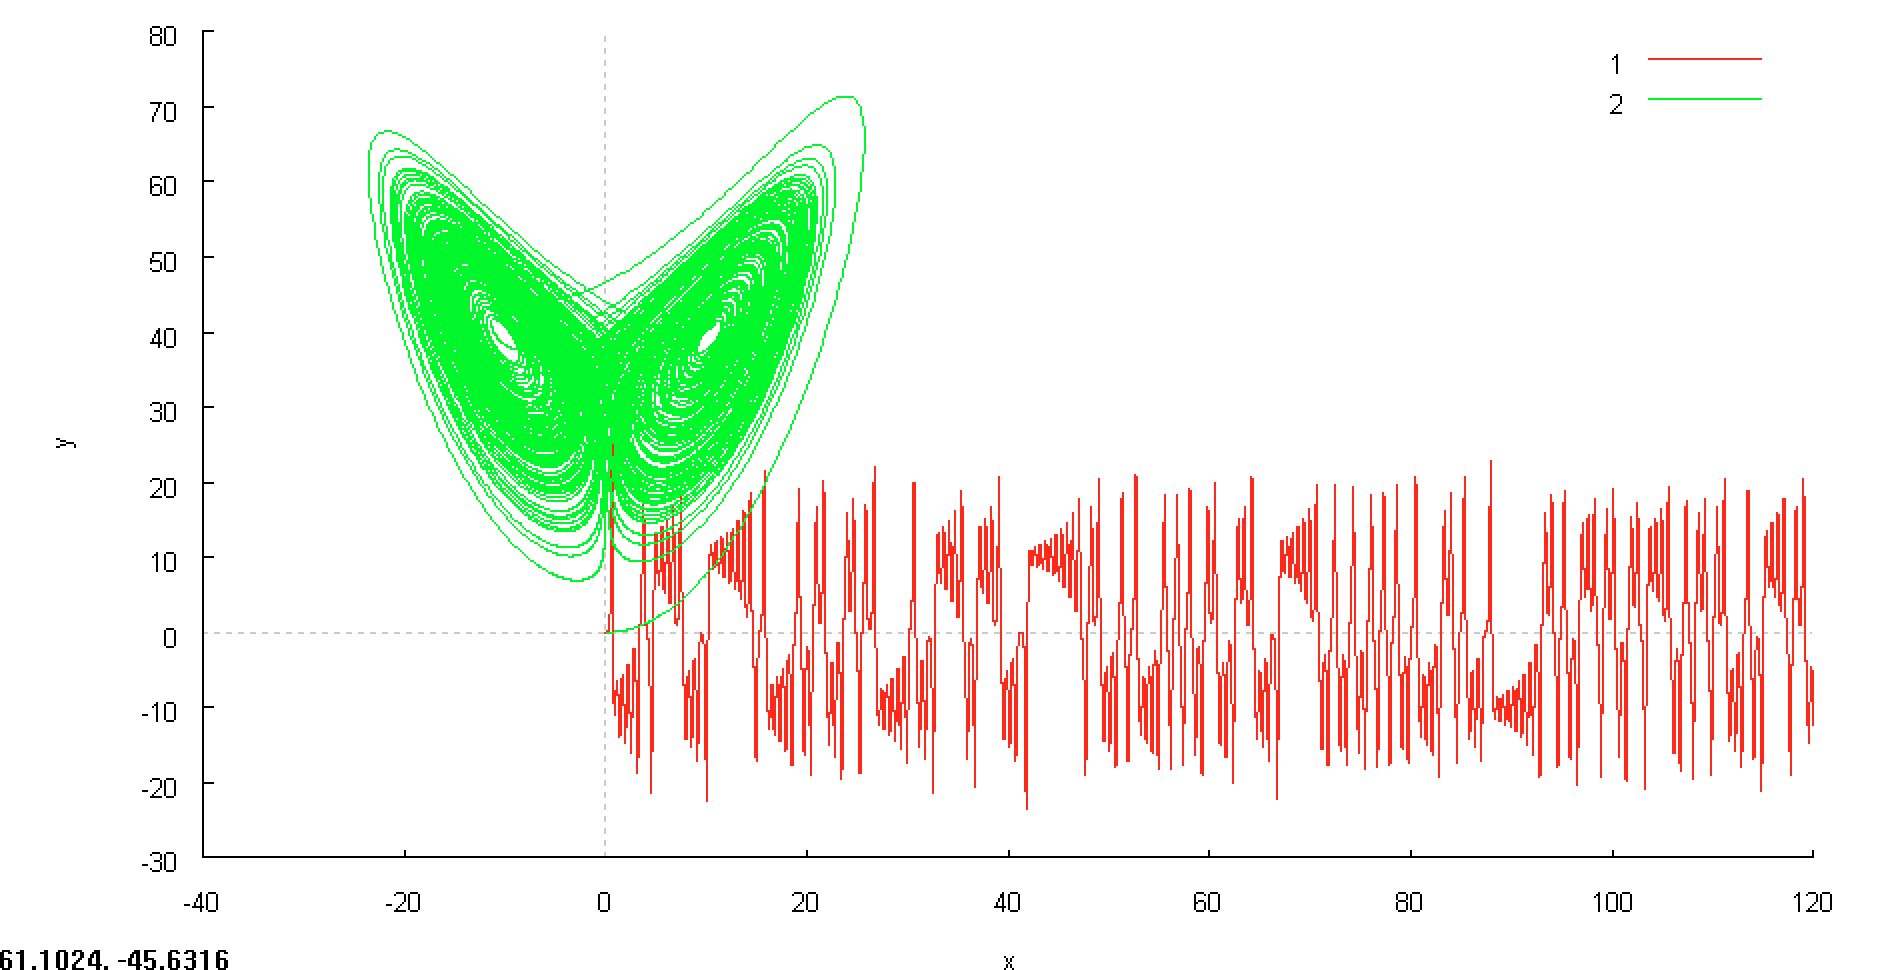
\includegraphics[width=0.9\linewidth]{../screenshots/lorenz.png}
\end{figure}

\begin{figure}[H]
\centering
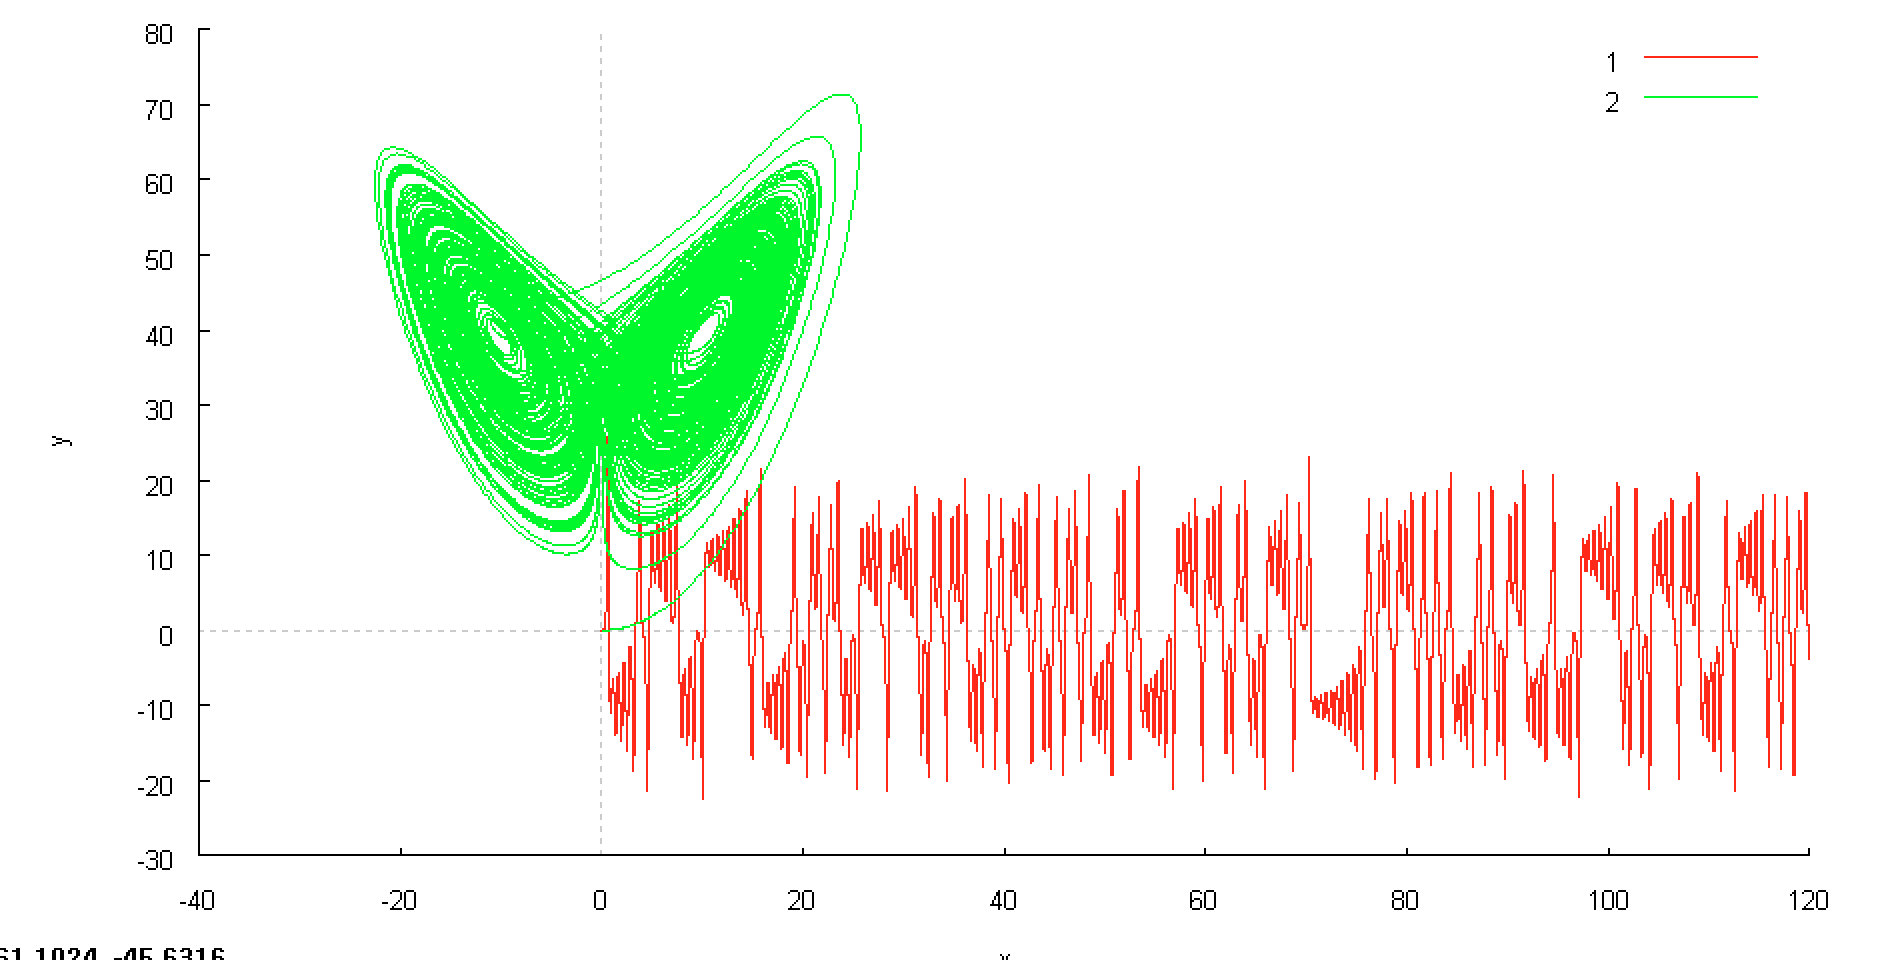
\includegraphics[width=0.9\linewidth]{../screenshots/lorenz000001.png}
\end{figure}


\subsection{Realisieren Sie das Differentialgleichungssystem mit MATLab/Simulink}

\begin{figure}[H]
\centering
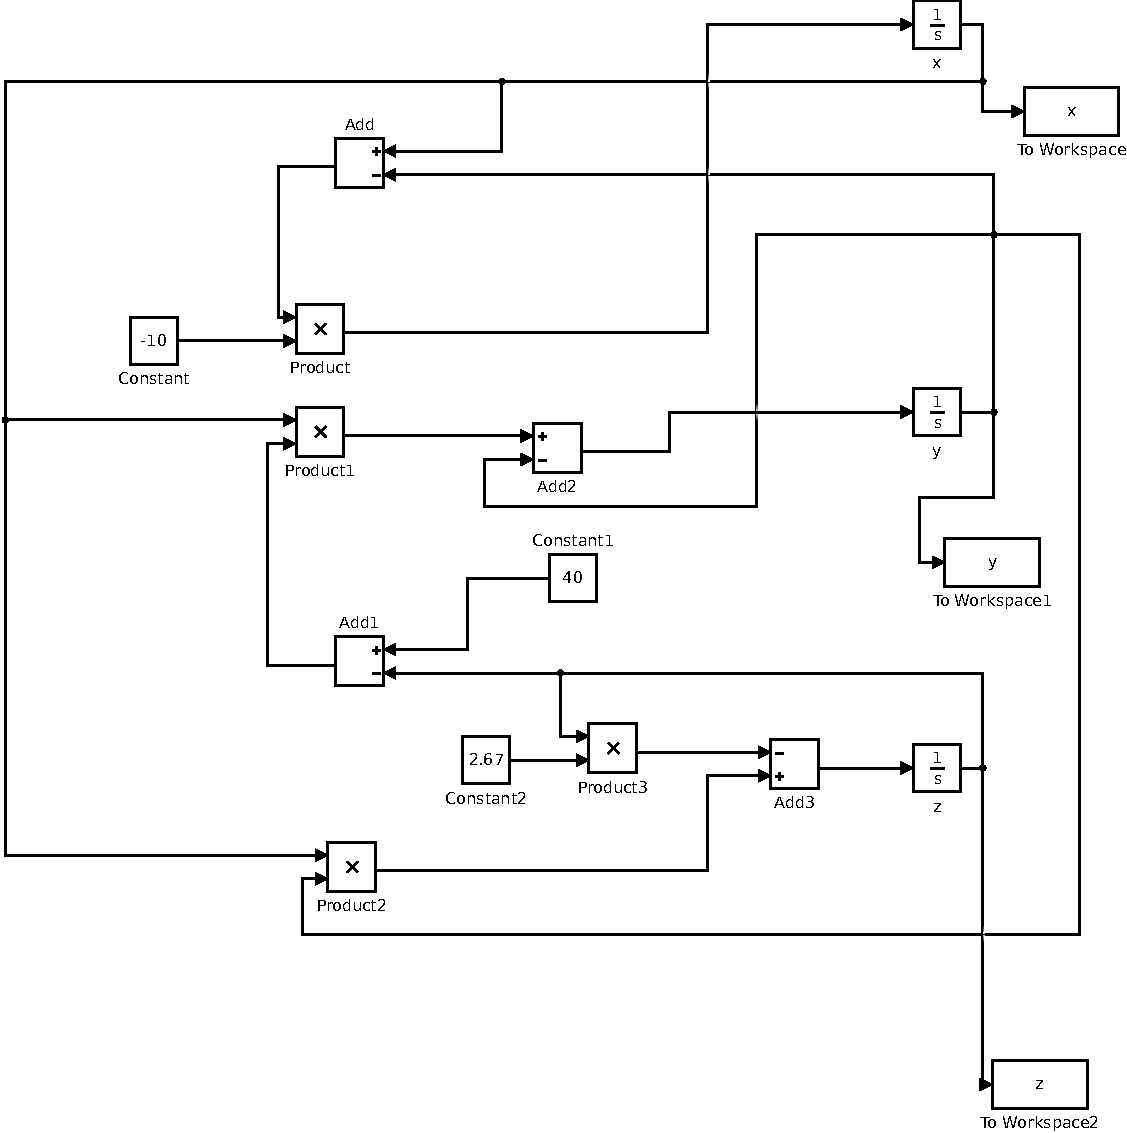
\includegraphics[width=0.9\linewidth]{../screenshots/3}
\end{figure}

Die Schmetterlingsdarstellung über den 3D Plotter, sieht wie folgt aus:

\begin{align}
plot3(x,y,z)
\end{align}
\begin{figure}[H]
\centering
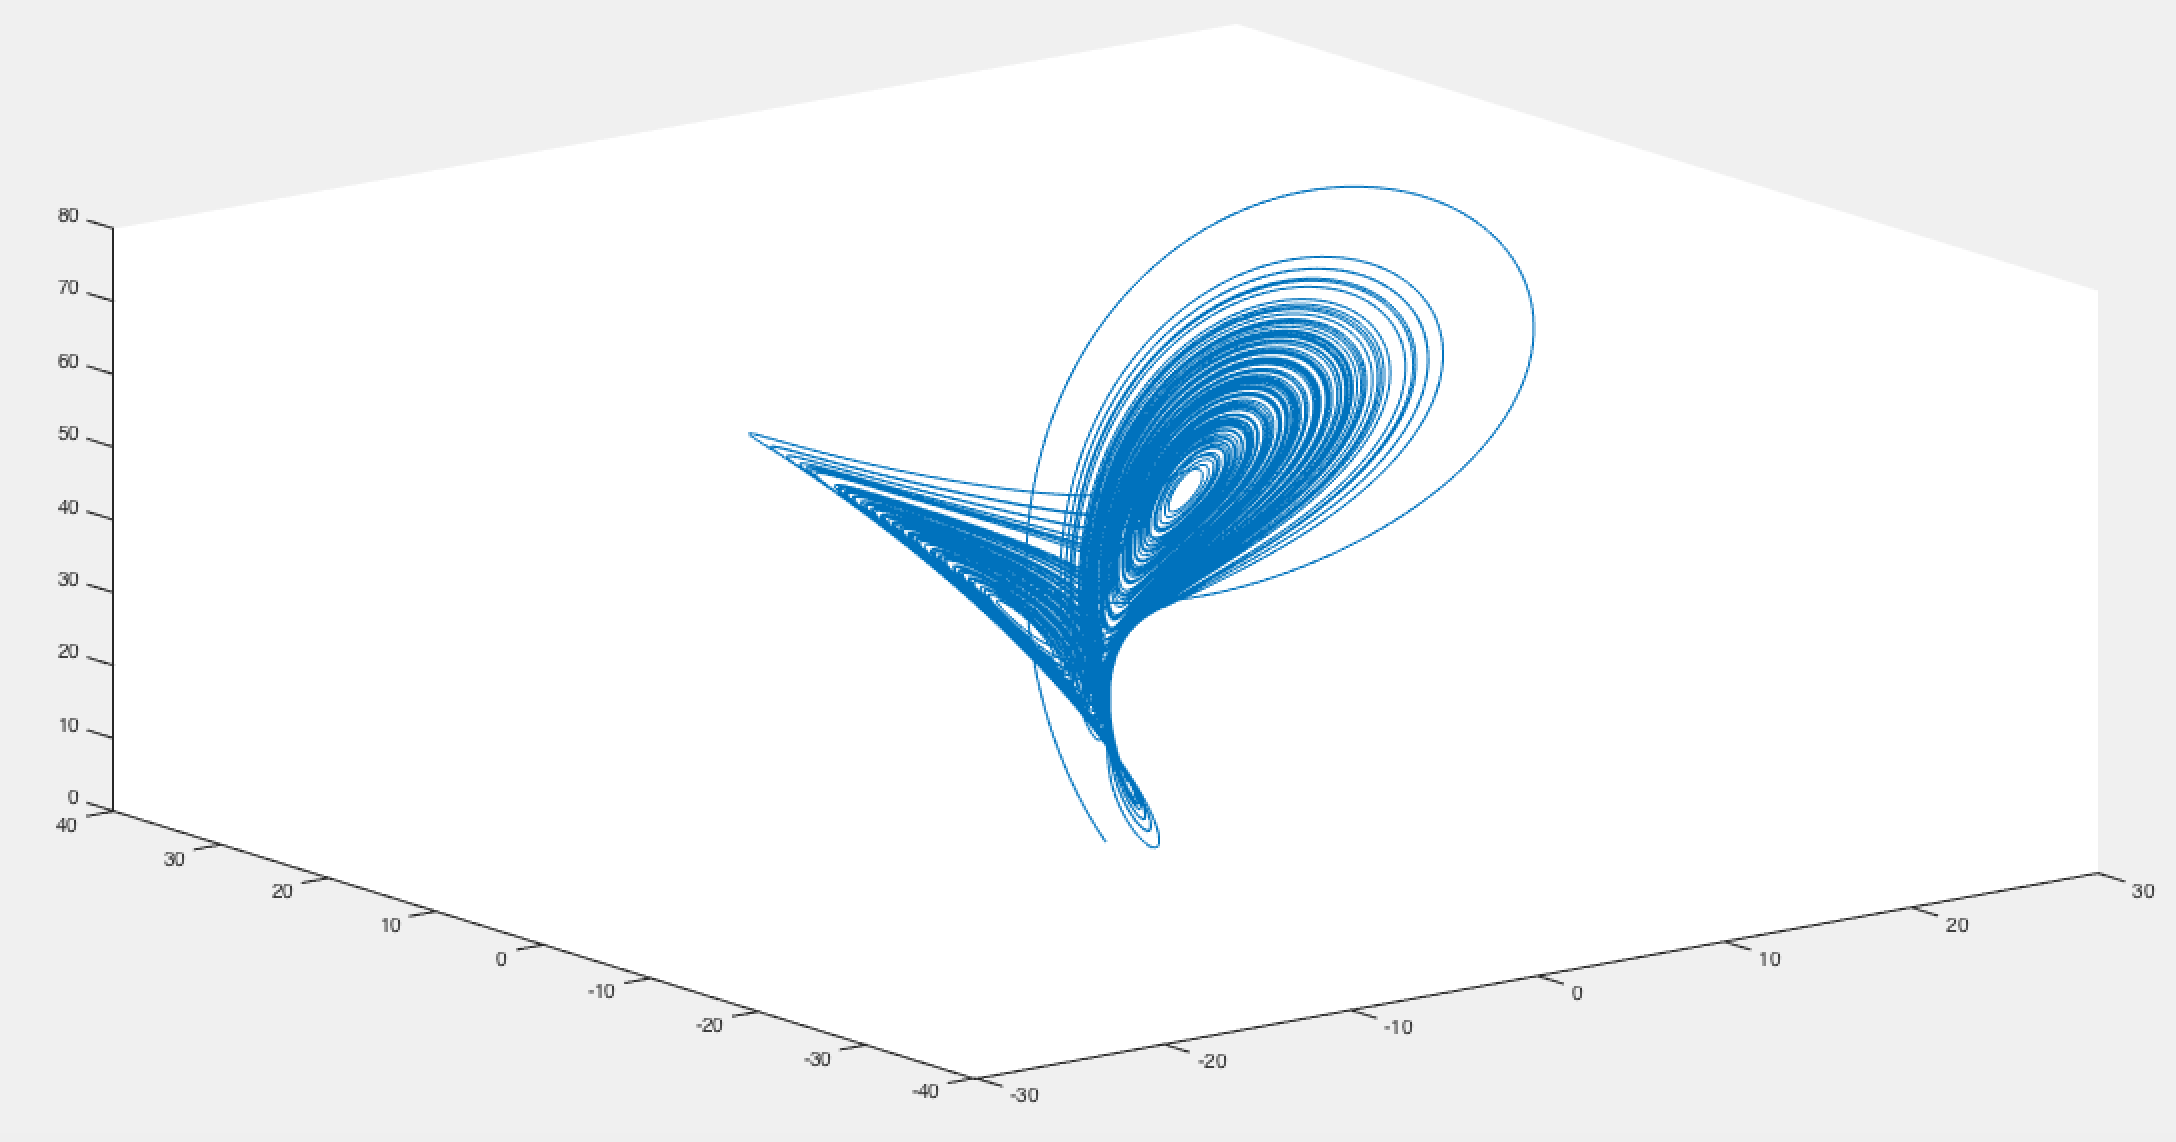
\includegraphics[width=0.9\linewidth]{../screenshots/lorenz_matlab.png}
\end{figure}

Wenn für die 2. Gleichung der Wert 40 (rot) in (40.000001) geändert wird (blau) und
die X-Werte in Relation zur Zeit jeweils geplottet werden, zeigt sich bis zu einem bestimmten X-wert (ca. 20) eine vollständige Überlagerung, danach laufen die Darstellungen  auseinander.

\begin{align}
plot(t,x,'blue')
\\hold \: on \nonumber
\\plot(t1,x1,'red') \nonumber
\end{align}

\begin{figure}[H]
\centering
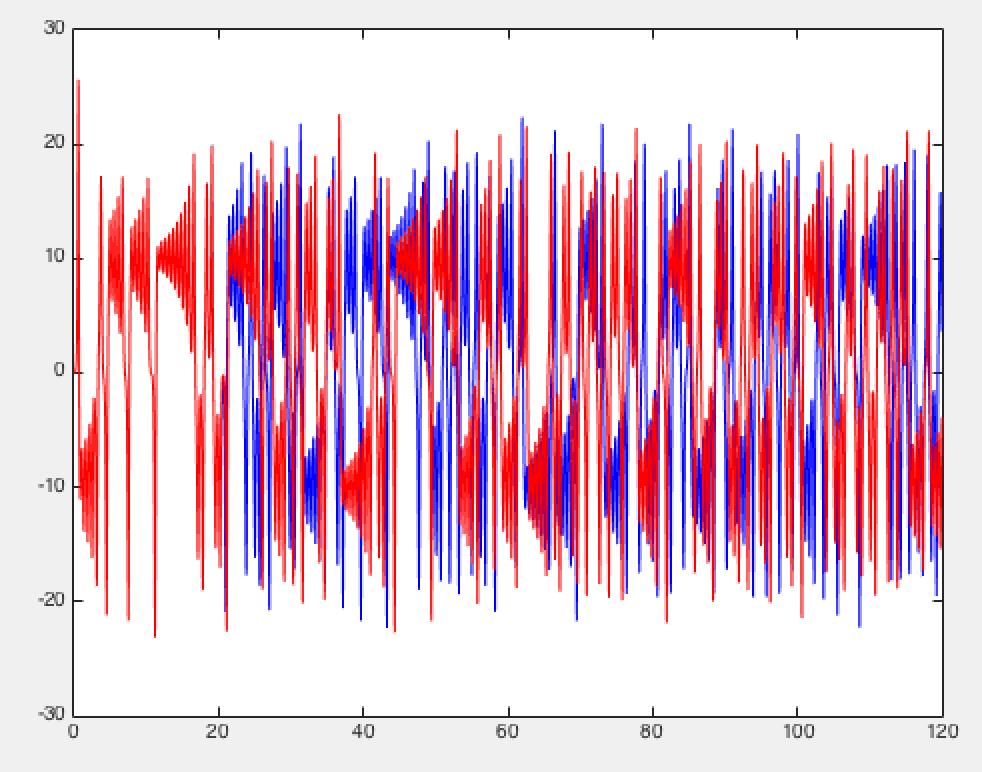
\includegraphics[width=0.9\linewidth]{../screenshots/lorenz_t.png}
\end{figure}

\end{document}